\documentclass[twocolumn, 10pt]{article}
\usepackage{amsmath}
\usepackage{graphicx}
\usepackage{caption}
\usepackage{float}
\usepackage{multicol}
\usepackage{tikz}
\usepackage{float}
\usepackage{geometry}

% Title and Author section formatting like you specifically?
\title{\textbf{Experimental Support for Newton’s Second Law}}
\author{Canada, C., D’Agostino, S., Fuks, E., Katz, J., Leung, R., Lee, E.}
\date{November 4, 2024} % No date

% Page layout
\setlength{\textwidth}{6.5in}
\setlength{\oddsidemargin}{0in}
\setlength{\evensidemargin}{0in}
\setlength{\topmargin}{-1in}
\setlength{\textheight}{9in}
\geometry{bottom = 0.75in, top = 0.6in}

\begin{document}
\twocolumn[
\begin{@twocolumnfalse}
    \maketitle
    \centering
    \begin{abstract}
The purpose of this experiment is to investigate the relationship between the net force and the acceleration of a system. This system was composed of a cart carrying varying masses connected by a string over a pulley to a counterweight. For each cart mass, three trials were conducted, and the time required for the cart to travel $0.5m$ was recorded. Acceleration was then calculated from this data. As the cart’s mass increased, its acceleration decreased, which showed the inverse relationship between mass and acceleration as stated by Newton's Second Law. These findings confirm that acceleration depends on both net force and mass, as described by  \(\vec{F} = m\vec{a}\).

     \end{abstract}
    \vspace{0.5cm}
\end{@twocolumnfalse}
]
\section*{INTRODUCTION}
\hspace{\parindent}The equation \(\sum\vec{F} = m\vec{a}\), commonly cited as Newton’s Second Law, represents a principle first written down by Sir Isaac Newton in his \textit{Principia} (1687), a principle that offers an explanation to how the motion of macroscopic systems can change. The equation directly relates the acceleration of a chosen system to the net force on that system. Here, force and acceleration are vector quantities, allowing the above equation to be applied separately to any set of directions one chooses. Thus, verifying Newton’s Second Law as a reasonable model would be valuable for deriving the masses or accelerations of bodies in nature.

If Newton’s Second Law is not accurate within our experiment's degree of precision:
\begin{equation} \label{eq1}
    H_0: \sum\vec{F} \neq m\vec{a}
\end{equation}

Alternatively, if Newton’s Second Law is accurate within our degree of precision:
\begin{equation} \label{NewtonsLaw} 
    H_A: \sum\vec{F} = m\vec{a} 
\end{equation}
\hspace{\parindent}
This lab investigated the relationship between force, mass, and acceleration through an experiment that utilized a two-mass pulley system. By setting up a cart connected to a hanging mass over a pulley and releasing it, the resulting acceleration of the carts and masses can then be observed and measured. We tested the null hypothesis by comparing the cart's measured accelerations (calculated via kinematics from multiple trials of data) to those predicted by net force equations originating from Newton's Second Law.

%conducting multiple trials and using the resulting data to calculate acceleration in two ways: using kinematic equations as a baseline method and applying net force equations from Newton’s Second Law as the method being tested.

 \section*{MATERIALS/METHODS}
 \begin{figure}[h]
    \centering
    \textbf{Fig. 1: Momentum Track Setup Used}
    \includegraphics[width=\columnwidth]{SetupPicture.png}
\end{figure}
\hspace{\parindent}The experiment used a 0.5 kg cart with low friction in its axles, allowing it to travel with minimal resistance across a smooth aluminum rail. In particular, the PASCO Dynamics Systems Basic Smart Cart Metal Track 1.2 m System and the PASCO Dynamics Systems Scientific ME-9454 Dynamic Collision Cart were used. The track was securely clamped to a level surface using Irwin trigger clamps. The cart, initially unloaded without any masses, was tied to a rope on the pulley with the small $0.02kg$ mass attached to the end. Starting from the 0.3m mark, the cart traveled to the 0.8m mark, traveling a total distance of 0.5m. A 0.5 kg mass was placed to indicate the stopping point. Three stopwatches and a metronome were used to time the different trials. These were used to improve the accuracy and reliability of timing measurements by syncing up the release of the cart and the start of the timers with the beat of the metronome. Trials were conducted three times per mass setting (1 kg, 2 kg, and 3 kg), incrementally adding 1 kg to the cart and keeping the small, hanging mass constant. This setup can be seen in Fig. 1.
\begin{figure}[H]
    \centering
    \textbf{Fig. 2. Free Body Diagram of the System}
\begin{tikzpicture} 
    % Cart
    \draw[fill=blue!20] (-3, 0) rectangle (-2, 0.5) node[midway] {$m_1$};
    \node at (-3.5, 0.25) {Cart}; % Mass label for cart
    
    % Horizontal surface for the cart
    \draw[thick] (-4, 0) -- (0.5, 0);
    
    % Pulley setup
    \draw[fill=gray!30] (0.7, 0) circle (0.25); % Horizontal pulley
    
    % String segments
    \draw[thick] (-2, 0.25) -- (0.775, 0.25); % String from cart to first pulley
    \draw[thick] (0.95, 0) -- (0.95, -3); % String from first pulley to second pulley
    
    % Hanging weight (m2)
    \node[draw, fill=red!20, minimum width=0.8cm, minimum height=0.8cm] at (1, -3.5) {$m_2$};
    
    % Force arrows on m1 (Cart)
    \draw[->, thick, red] (-2.5, 0.5) -- ++(0, 1) node[anchor=south] {$N$}; % Normal force
    \draw[->, thick, red] (-2.5, 0) -- ++(0, -1) node[anchor=north] {$m_1 g$}; % Weight of the cart
    \draw[->, thick, blue] (-2, 0.25) -- ++(0.75, 0) node[anchor=south] {$T$}; % Tension
    
    % Force arrows on m2 (Hanging weight)
    \draw[->, thick, red] (0.95, -3.9) -- ++(0, -1) node[anchor=east] {$m_2 g$}; % Gravity on hanging weight
    \draw[->, thick, blue] (0.95, -3.1) -- ++(0, 0.75) node[anchor=east] {$T$}; % Tension
    
    \draw[->, thick, black] (-1, 1.5) -- ++(1, 0);
    \node at (-0.5, 1.75) {+ acceleration};
    
    % Labels for pulleys
    \node at (1.5, 0.5) {Pulley 1};


\end{tikzpicture}
\end{figure}


\section*{RESULTS}
\begin{figure} [h]
    \centering
    \textbf{Fig. 3: Time to Accelerate 0.5m vs. Mass of Cart/Weight System - Square Root Fit}
    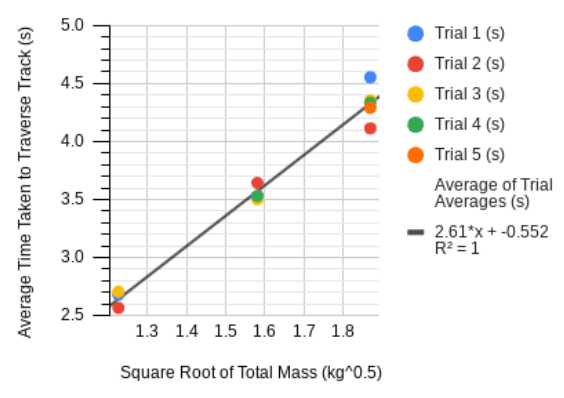
\includegraphics[width=\columnwidth]{Time vs. Mass (Square Root Fit).png}
    \text{Theoretical Relation: $t=(\sqrt{\frac{2\Delta x}{||\sum\vec{F}||}})(\sqrt{m})$}
\end{figure}
\begin{figure}
    \centering
    \textbf{Fig. 4: Cart System Acceleration vs. Reciprocal Mass}
    \includegraphics[width=\columnwidth]{Acceleration vs. Reciprocal Mass.png}
    \label{fig:Square Root Fit}
\end{figure}

\hspace{\parindent} A plot of the average travel times for the cart and its load versus the mass of the cart and load is shown in Fig. 3. Note that each trial utilized three timers for each mass, and so each point is the mean of three times. Various regressions were fitted to the data (via the least square method; see Discussion), with the closest best-fit line shown in Fig. 3 (a square root regression).

Newton's Second Law (Experimental Method): 
\begin{equation} \label{Dynamics}
    \sum\vec{F} = m\vec{a}
\end{equation}

 Kinematics (Baseline Method): 
\begin{equation} \label{Kinematics}
    \vec{x}(t) = \vec{x}_0 + \vec{v}_0t + \frac{1}{2}\vec{a} t^2
\end{equation}

Doing the calculations using a 1 kg weight will result in the following calculations (which correspond to the first cluster of points in Fig. 3:

Using our data in Equation~\eqref{Kinematics}: 
\begin{gather*}
    x(t) = 0.5m
    \\x_0 = 0m
    \\v_0 = 0m/s
    \\t = 2.65s
    \\0.5\text{m} = (0\text{m}) + (0\text{m/s})(2.65\text{s})+\frac{1}{2}(a)(2.65\text{s})^2
    \\a = (1/2.65)^2\text{m}/\text{s}^2
    \\a = 0.1424\text{m}/\text{s}^2
\end{gather*}

A free body diagram (see Fig 2.) can be drawn of the system with the momentum cart (\(m_1\)) and the falling mass (\(m_2\)). A system of equations can be created by applying Equation ~\eqref{Dynamics} to the vectors along the perpendicular axis indicated in Fig. 2. The string and pulley are assumed to have both negligible mass and friction, thus both tension forces are approximately equal, simplifying calculations. The calculation of \(a\) is shown below (for more on this system, see Tipler and Mosca).
\begin{gather*}
     \\m_1 = 1.5 kg, \quad m_2 = 0.02kg, \quad g , = 9.8m/s^2
    \\ \sum\vec{F}=m\vec{a}\Rightarrow
    \\T = m_1a, \tag{5}
    \\m_2a = m_2g - T \tag{6}
    \\ \Rightarrow T = m_2g - m_2a \Rightarrow m_1a =  m_2g - m_2a
    \\ \Rightarrow m_1a + m_2a = m_2g \Rightarrow a(m_1 + m_2) = m_2g 
    \\ \Rightarrow a = \frac{m_2g}{m_1 + m_2} \tag{7}
    \\ \Rightarrow a = \frac{0.02\text{kg}*9.8\text{m}/\text{s}^2}{0.02\text{kg}+1.5\text{kg}} \approx 0.129 m/s^2 
\end{gather*}


An \(a\) of \(0.1424 m/s^2\) calculated through kinematics and is relatively close to our \(a\) of \(0.129 m/s^2\) calculated through \(\sum\vec{F} = m\vec{a}\). The percent error is:
\begin{gather*}
    \left\lvert \frac{a_{calculated}-a_{experimental}}{a_{calculated}} \right\rvert = \tag{8}
    \\\frac{0.1424 m/s^2-0.129m/s^2}{0.1424 m/s^2} \approx 0.094 = 9.4\%
\end{gather*}
just under 10\%. Repeating the above calculations for 2 kg and 3 kg mass loads ($m_1=2.5$ and $3.5$, respectively) using both kinematics and force equations yields similar percent errors of about 2.1\% and 4.2\%, well within the acceptable 10\% range for experimental uncertainty. Fig. 4 is a plot of these accelerations versus the cart system's mass.



\section*{DISCUSSION}
\hspace{\parindent} The variables directly measured in the experiment (mass and time) were plotted in Fig. 3 with a corresponding square root regression. From the coefficient of determination in Fig. 3 ($R^2=1$), the data is consistent with direct proportionality between the time traveled and the square root of the cart system's mass. That proportionality comes from substituting the simplified kinematic relation between time and displacement $\Delta x=\frac{1}{2}at^2$ into Newton's Second Law (see Fig. 3 for exact relation). This is further supported by an $R^2$ value of 1 in Fig. 4, which directly suggests that the cart system's acceleration was directly proportional to its reciprocal mass as predicted by Newton's Second Law (where the constant of proportionality is $||\sum\vec{F}||$). As mentioned under Results, other regressions were tested to see whether they could fit the data better than square root and linear correlations, respectively, and thus invalidate the accuracy of Newton's Second Law. Exponential and logarithmic regressions, however, both had slightly poorer $R^2$ values for Fig. 3 data ($0.998$ and $0.994$, respectively) and Fig. 4 data ($0.992$ and $0.989$), suggesting that their high values are merely a result of insufficient data points. (Higher order polynomials will trivially have perfect correlations, and thus do not disprove our hypothesis).

\hspace{\parindent} The acceleration derived through (Newtonian) mechanics differed measurably from that calculated through kinematics due to several potential sources of experimental error. For one, more trials with different masses would be required to more definitively characterize the seemingly optimal regressions in Fig. 3 as square root and Fig. 4 as linear rather than exponential, logarithmic, or any other relationship. Also, the experimental set-up may have had significant friction in various places, such as axial friction in the wheels and pulley or static friction between the rope and the pulley, forces that were not accounted for when acceleration was calculated using Newton's Second Law. Axial friction, for example, would have rendered the tension forces acting on the cart and counterweight to be unequal, likely reducing the overall acceleration of the system. Another potential source of significant error was the human error associated with our timing methods. Instead of relying on the reaction speeds of the timers responding to the metronome, a more accurate method might have employed electronics (e.g. camera sensors) to ensure the timers began their stopwatches at the same exact instant that the cart was released.
\section*{CONCLUSION}
\hspace{\parindent}In supporting Newton's Second Law, our findings reinforce the validity of a key part of classical mechanics by showing correlation between mass and acceleration. This knowledge helps us understand systems varying from moving cars to orbiting satellites, illustrating its utility in describing and predicting everyday phenomena, advanced engineering and design situations, and potentially many other scientific and technological fields. For example, Newton's Second Law is integral to mechanical engineering, where it informs the design of machinery and vehicles, and to civil engineering, where it helps with structural analysis and load distribution (by assuming acceleration in $\sum \vec{F}=m\vec{a}$ is zero), thus ensuring the stability of buildings and bridges. Moreover, confirming Newton's Second Law opens the way to developing more sophisticated and useful formalizations of mechanics that align with it.




\section*{Resources/Bibliography}
[1] I. Newton, Philosophiæ Naturalis Principia Mathematica (1687).

\noindent[2] P.A. Tipler, and G. Mosca, Physics for Scientists and Engineers (Macmillan Higher Education, 2007).



\section*{ACKNOWLEDGMENTS} 
Thank you to C. Canada, S. D’Agostino, E. Fuks, J. Katz, E. Lee, and R. Leung for working on the lab and writing the report.

Thank you to all peer reviewers (including the chief editor, Dr. Evangelista) of the Journal of Science and Engineering for the constructive feedback that helped to greatly improve this paper.

\end{document}
